\chapter{Hardware Limitations on Screen Reader/Magnifier Latency}\label{vision-assistive-technology-laptop-computer-requirements}
\raggedright
\section{Executive Summary}\label{executive-summary}

Screen reader\index{screen reader} response latency—the delay between user input\index{screen reader!user input} and audio feedback—creates significant barriers to academic success for students using assistive technology\index{assistive technology} on underpowered computers.\supercite{Foley2017AssistiveTechnologyOutcomes} Research demonstrates that hardware\index{hardware} limitations, particularly insufficient RAM\index{RAM} and older CPU generations, directly increase response delays that trigger frustration, impair task completion, and ultimately undermine educational outcomes.\supercite{Kelly2011, StudentOutcomesResearch} Current findings indicate that systems with 16 GB RAM\index{RAM} demonstrate unacceptably long latency\index{latency} periods, necessitating a minimum recommendation of 24-32 GB RAM for educational equity\index{educational equity}. See Appendix~\ref{chap:computationappendix} for the supporting data.

\section{The Latency Problem}\label{the-latency-problem}

\subsection{The Zero-Frustration Imperative}\label{the-zero-frustration-imperative}

\subsubsection{Equivalent Response Times}

Students using screen readers must achieve equivalent response times to their sighted peers to ensure educational equity\index{educational equity}. Any additional latency beyond what sighted users experience creates an unfair disadvantage and violates principles of equal access.\supercite{ADA1990, Section508}

\subsection{Critical Response Time Thresholds}\label{critical-response-time-thresholds}

\subsubsection{Perceptibility Thresholds:}

\begin{itemize}
	\item \textbf{<10 ms}: Imperceptible, maintaining illusion of instantaneous response (TARGET RANGE) \supercite{Nielsen1993UsabilityEngineering}
	\item \textbf{10-100 ms}: Noticeable delay disrupts user flow, causes mild frustration \supercite{Miller1968ReactionTime}
	\item \textbf{>100 ms}: Consistently interrupts interaction flow, prompts repeated inputs \supercite{Shneiderman1998DesigningTheUserInterface}
\end{itemize}


\subsubsection{Frustration Thresholds:}

\begin{itemize}
	\item \textbf{100-500 ms}: Significant frustration in direct manipulation tasks, degrades efficiency and increases errors \supercite{Card1983ThePsychologyOfHumanComputerInteraction}
	\item \textbf{>500 ms}: Unacceptable for educational use—users abandon tasks due to perceived system freezes \supercite{Sears1993TheEffectOfResponseTime}
	\item \textbf{>1 second}: Severely disrupts attention and learning flow \supercite{Dix2004HumanComputerInteraction}
\end{itemize}


\subsubsection{Audio-Specific Critical Factors:}

\begin{itemize}
	\item \textbf{20 ms}: Lower threshold for audible delay perception in screen reader\index{screen reader} audio feedback \supercite{Grunwald1999AuditoryLatency}
	\item \textbf{25 ms}: Performance degradation threshold—beyond this point, measurable efficiency loss occurs \supercite{Fowler2011ScreenReaderLatency}
	\item \textbf{100-800 ms}: Critical danger zone where speech truncation occurs, causing navigation errors and forcing workflow adjustments \supercite{Bigham2014UnderstandingScreenReaderUsage}
\end{itemize}


\subsubsection{Educational Equity Standard:}

For true accessibility, screen reader response times must remain \textbf{under 25 ms} to match the responsiveness sighted students experience with visual interfaces \supercite{W3C2018WCAG21}.

\subsection{Hardware Impact on Response Times}\label{hardware-impact-on-response-times}

Older processors and limited system RAM\index{RAM} substantially increase keypress-to-audio output delays through several mechanisms:

\subsubsection{Memory Constraints:}

\begin{itemize}
	\item Insufficient \gls{ram} forces reliance on slower storage (page files) \supercite{Microsoft2023WindowsPerformance}
	\item Creates noticeable lags during multitasking \supercite{Intel2024ProcessorMemory}
	\item Causes \gls{audio} stuttering when memory-intensive applications run \supercite{Realtek2023AudioDriverPerformance}
\end{itemize}


\subsubsection{Processor Limitations:}

\begin{itemize}
	\item Older CPUs have slower data processing speeds \supercite{AMD2024RyzenPerformance}
	\item Less efficient memory controllers delay data transfer \supercite{AnandTech2023MemoryControllers}
	\item Higher CAS latency\index{latency} in older RAM configurations compounds delays \supercite{TechSpot2023RAMTimings}
\end{itemize}


\subsubsection{Audio System Factors:}

\begin{itemize}
	\item Generic audio drivers introduce additional \gls{latency} \supercite{ASIO4ALL2023Latency}
	\item OS-level buffering creates inherent delays \supercite{LinuxAudioLatency}
	\item Power-saving modes cause inconsistent response times \supercite{WindowsPowerManagement}
\end{itemize}


\section{Educational Impact}\label{educational-impact}

\subsection{Academic Performance Degradation}\label{academic-performance-degradation}

The combination of hardware\index{hardware} limitations and increased latency creates cascading effects on student learning:

\subsubsection{Cognitive Load Increase:}
\begin{itemize}
	\item Students must wait for audio feedback before proceeding \supercite{Sweller1988CognitiveLoadTheory}
	\item Disrupted information flow breaks concentration \supercite{Parasuraman2008CognitiveWorkload}
	\item Increased mental effort required for basic \gls{navigation} tasks \supercite{Wickens2008MultipleResourceTheory}
\end{itemize}

\subsubsection{Task Completion Barriers:}

\begin{itemize}
	\item Time-pressured assignments become difficult or impossible \supercite{Adams2000ImpactOfTechnology}
	\item Complex multi-step tasks are abandoned due to lag \supercite{Kirschner2006WhyMinimalGuidance}
	\item Workflow interruptions prevent deep engagement with content \supercite{Pashler1994DualTaskInterference}
\end{itemize}

\subsubsection{Comprehension Challenges:}

\begin{itemize}
	\item Broken information flow leads to shallow processing \supercite{Craik1972LevelsOfProcessing}
	\item Reduced attention and increased mind-wandering \supercite{Smallwood2011MindWandering}
	\item Lower retention compared to smooth, responsive interactions \supercite{Kintsch1998Comprehension}
\end{itemize}

\subsection{Emotional and Psychological Consequences}\label{emotional-and-psychological-consequences}

Students experiencing screen reader\index{screen reader} latency report specific negative emotional reactions:

\subsubsection{Immediate Responses:}

\begin{itemize}
	\item \textbf{Frustration}: Escalating as delays persist and disrupt workflow \supercite{Lazarus1991EmotionAndAdaptation}
	\item \textbf{Anger}: When perceiving latency as unfair obstacle to achievement \supercite{Fogg2003PersuasiveTechnology}
	\item \textbf{Anxiety}: Fear of missing deadlines or failing to complete work \supercite{Zeidner1998TestAnxiety}
\end{itemize}


\subsubsection{Sustained Impact:}

\begin{itemize}
	\item \textbf{Stress}: Elevated levels impairing cognitive function \supercite{Sapolsky2004WhyZebrasDontGetUlcers}
	\item \textbf{Helplessness}: Feeling unable to control technical barriers \supercite{Seligman1975Helplessness}
	\item \textbf{Shame}: Particularly when singled out or falling behind peers \supercite{Brown2010TheGiftsOfImperfection}
\end{itemize}


These emotional responses create additional barriers to learning, as stress and anxiety further impair working memory and concentration \supercite{Eysenck2007AnxietyAndCognition}.

\section{The Digital Divide Effect}\label{the-digital-divide-effect}

Hardware\index{hardware}-induced latency disproportionately affects students with limited resources:

\begin{itemize}
	\item Students using older or cheaper devices experience higher latency\index{latency} \supercite{Attewell2001TheDigitalDivide}
	\item Cannot afford hardware\index{hardware} upgrades to improve performance \supercite{Warschauer2003TechnologyAndSocialInclusion}
	\item Fall further behind academically due to technical barriers \supercite{DiMaggio2001FromUnequalAccess}
	\item May abandon computer-based tasks or courses entirely \supercite{Compaine2001TheDigitalDivide}
\end{itemize}

\section{RAM-Specific Impact Analysis}\label{ram-specific-impact-analysis}

\subsection{RAM-Specific Performance Against Zero-Frustration Standard}\label{ram-specific-performance-against-zero-frustration-standard}

Screen readers require consistent sub-25ms response times to achieve parity with sighted user experiences. Current RAM\index{RAM} configurations perform as follows against this critical standard:

\subsubsection{8GB RAM Systems - FAILS EQUITY STANDARD:}

\begin{itemize}
	\item \textbf{Typical Latency}: 150-400ms during educational multitasking \supercite{InternalTestingData2024}
	\item \textbf{Peak Latency}: Up to 800ms when memory saturated \supercite{InternalTestingData2024}
	\item \textbf{Equity Gap}: 6-32x slower than acceptable threshold \supercite{EquityAnalysisRevision}
	\item \textbf{Educational Impact}: Creates insurmountable barrier to equal participation \supercite{EducationalEquityReport2024}
\end{itemize}


\subsubsection{16GB RAM Systems - UNACCEPTABLY INADEQUATE:}

\begin{itemize}
	\item \textbf{Typical Latency}: 125-300ms under normal educational workloads \supercite{InternalTestingData2024}
	\item \textbf{Peak Latency}: 450ms during intensive multitasking \supercite{InternalTestingData2024}
	\item \textbf{Equity Gap}: 5-12x slower than equity standard \supercite{EquityAnalysisRevision}
	\item \textbf{Educational Impact}: Demonstrates unacceptably long latency\index{latency} that severely impairs educational performance and violates accessibility\index{accessibility} standards \supercite{EducationalEquityReport2024}
\end{itemize}


\subsubsection{24GB RAM Systems - MINIMUM THRESHOLD:}

\begin{itemize}
	\item \textbf{Typical Latency}: 75-150ms consistently \supercite{InternalTestingData2024}
	\item \textbf{Peak Latency}: 200ms under moderate load \supercite{InternalTestingData2024}
	\item \textbf{Equity Gap}: 3-6x slower than ideal, approaching minimum acceptable \supercite{EquityAnalysisRevision}
	\item \textbf{Educational Impact}: Represents minimum viable configuration for educational equity\index{educational equity} \supercite{EducationalEquityReport2024}
\end{itemize}


\subsubsection{32GB RAM Systems - APPROACHES EQUITY:}

\begin{itemize}
	\item \textbf{Typical Latency}: 50-100ms consistently \supercite{InternalTestingData2024}
	\item \textbf{Peak Latency}: 150ms under extreme load \supercite{InternalTestingData2024}
	\item \textbf{Equity Gap}: 2-4x slower than ideal, within reasonable tolerance \supercite{EquityAnalysisRevision}
	\item \textbf{Educational Impact}: Minor but measurable disadvantage, approaching acceptable performance \supercite{EducationalEquityReport2024}
\end{itemize}


\subsubsection{64GB RAM Systems - ACHIEVES EQUITY STANDARD:}

\begin{itemize}
	\item \textbf{Typical Latency}: 40-75ms (primarily limited by CPU\index{CPU}/storage) \supercite{InternalTestingData2024}
	\item \textbf{Peak Latency}: Under 100ms even under heavy load \supercite{InternalTestingData2024}
	\item \textbf{Equity Gap}: 1.5-3x slower, within reasonable tolerance \supercite{EquityAnalysisRevision}
	\item \textbf{Educational Impact}: Essentially equivalent to sighted user experience \supercite{EducationalEquityReport2024}
\end{itemize}


\subsection{The Equity Crisis Revealed}\label{the-equity-crisis-revealed}

Using the zero-frustration standard exposes the severity of the \gls{educationalequity} problem:

\begin{itemize}
	\item \textbf{Students with 8GB systems}: Experience 6-32x longer response times than necessary for equal access \supercite{EducationalEquityReport2024}
	\item \textbf{Students with 16GB systems}: Still face unacceptably long latency with 5-12x disadvantage compared to equity standard \supercite{EducationalEquityReport2024}
	\item \textbf{Students require 24-32GB systems minimum}: To begin approaching true educational equity\index{educational equity} for screen reader\index{screen reader} users \supercite{EducationalEquityReport2024}
	\item \textbf{Only 32GB+ systems}: Achieve performance levels that approach acceptable educational equity standards \supercite{EducationalEquityReport2024}
\end{itemize}


\hypertarget{hardware\index{hardware}-configuration-analysis}{}\section{Hardware Configuration Analysis}\label{hardware-configuration-analysis}
\subsection{Comprehensive System Performance Against Equity Standard}\label{comprehensive-system-performance-against-equity-standard}

\footnotesize

\begin{longtblr}[
		caption = {Comprehensive system performance against equity standard},
		label = {tab:chapter1:system-performance},
		note = {This table compares various system types and hardware configurations against the equity standard for educational technology. It highlights how RAM, CPU generation, and latency impact compliance with accessibility\index{accessibility} standards and educational viability, providing a detailed overview of which configurations meet or violate equity requirements.},
	]{
		colspec = {X[l,m] X[l,m] X[l,m] X[l,m] X[l,m] X[l,m]},
		rowhead = 1,
		row{1} = {font=\normalfont},
		hlines,
		stretch = 1.5
	}
	System Type          & RAM\index{RAM} Level & CPU Generation              & Typical Latency & Equity Compliance\index{accessibility!legal accessibility}      & Educational Viability                                                                                       \\
	Budget Systems       & 4-8GB                & 2nd-4th Gen Intel/AMD FX    & 300-1000+ ms    & FAILS (12-40x slower) \supercite{InternalTestingData2024}       & Violates accessibility\index{accessibility} standards \supercite{EducationalEquityReport2024}               \\
	Entry Educational    & 8GB                  & 6th-8th Gen Intel/Ryzen 2   & 150-400 ms      & FAILS (6-16x slower) \supercite{InternalTestingData2024}        & Creates substantial educational barrier \supercite{EducationalEquityReport2024}                             \\
	Standard Educational & 16GB                 & 8th-10th Gen Intel/Ryzen 3  & 125-300 ms      & UNACCEPTABLE (5-12x slower) \supercite{InternalTestingData2024} & Demonstrates unacceptably long latency\index{latency} \supercite{EducationalEquityReport2024}               \\
	Minimum Viable       & 24GB                 & 10th+ Gen Intel/Ryzen 5     & 75-150 ms       & THRESHOLD (3-6x slower) \supercite{InternalTestingData2024}     & Minimum acceptable for educational equity\index{educational equity} \supercite{EducationalEquityReport2024} \\
	Enhanced Educational & 32GB                 & 10th+ Gen Intel/Ryzen 5+    & 50-100 ms       & APPROACHING (2-4x slower) \supercite{InternalTestingData2024}   & Minor but measurable disadvantage \supercite{EducationalEquityReport2024}                                   \\
	Equity-Compliant     & 64GB                 & Latest Gen High-Performance & 15-50 ms        & ACHIEVES (≤2x slower) \supercite{InternalTestingData2024}       & True educational equity\index{educational equity} \supercite{EducationalEquityReport2024}                   \\
\end{longtblr}
\normalsize


\subsection{Zero-Frustration Performance Benchmarks}\label{zero-frustration-performance-benchmarks}

To achieve educational equity, systems must consistently deliver:

\subsubsection{Target Performance Metrics:}

\begin{itemize}
	\item \textbf{Keystroke Response}: <25ms from keypress to audio feedback \supercite{W3C2018WCAG21}
	\item \textbf{Navigation Commands}: <20ms for arrow key/tab navigation \supercite{Fowler2011ScreenReaderLatency}
	\item \textbf{Application Switching}: <50ms maximum delay \supercite{Nielsen1993UsabilityEngineering}
	\item \textbf{Document Loading}: <100ms for typical educational documents \supercite{Shneiderman1998DesigningTheUserInterface}
	\item \textbf{Web Page Reading}: <30ms between elements during continuous reading \supercite{Bigham2014UnderstandingScreenReaderUsage}
\end{itemize}


\subsubsection{Current System Performance Against Benchmarks:}

\subsubsection{8GB Systems - EDUCATIONAL EQUITY VIOLATION:}

\begin{itemize}
	\item Keystroke response: 150-400ms (\textbf{6-16x too slow}) \supercite{InternalTestingData2024}
	\item Navigation: 200-500ms (\textbf{8-20x too slow}) \supercite{InternalTestingData2024}
	\item App\index{apps} switching: 300-800ms (\textbf{6-16x too slow}) \supercite{InternalTestingData2024}
	\item \textbf{Result}: Creates insurmountable educational disadvantage \supercite{EducationalEquityReport2024}
\end{itemize}


\subsubsection{16GB Systems - UNACCEPTABLY INADEQUATE:}

\begin{itemize}
	\item Keystroke response: 125-300ms (\textbf{5-12x too slow}) \supercite{InternalTestingData2024}
	\item Navigation: 150-350ms (\textbf{6-14x too slow}) \supercite{InternalTestingData2024}
	\item App switching: 200-450ms (\textbf{4-9x too slow}) \supercite{InternalTestingData2024}
	\item \textbf{Result}: Demonstrates unacceptably long latency that prevents educational equity \supercite{EducationalEquityReport2024}
\end{itemize}


\subsubsection{24GB Systems - MINIMUM THRESHOLD:}

\begin{itemize}
	\item Keystroke response: 75-150ms (\textbf{3-6x too slow}) \supercite{InternalTestingData2024}
	\item Navigation: 90-200ms (\textbf{3.6-8x too slow}) \supercite{InternalTestingData2024}
	\item App switching: 100-200ms (\textbf{2-4x too slow}) \supercite{InternalTestingData2024}
	\item \textbf{Result}: Represents minimum viable performance for educational settings \supercite{EducationalEquityReport2024}
\end{itemize}


\subsubsection{32GB+ Systems - APPROACHES EQUITY:}

\begin{itemize}
	\item Keystroke response: 30-75ms (\textbf{1.2-3x slower than ideal}) \supercite{InternalTestingData2024}
	\item Navigation: 25-60ms (\textbf{1.2-2.4x slower than ideal}) \supercite{InternalTestingData2024}
	\item App switching: 50-120ms (\textbf{1-2.4x slower than ideal}) \supercite{InternalTestingData2024}
	\item \textbf{Result}: Minor efficiency loss, approaching true equity \supercite{EducationalEquityReport2024}
\end{itemize}


\hypertarget{measured-performance-data}{}\section{Measured Performance Data}\label{measured-performance-data}

\subsection{Screenreader Loading Latency}\label{screenreader-loading-latency}

The latency of a screenreader\index{screen reader} is the time it takes for the software\index{software} to load and start functioning. Insufficient RAM can cause the screenreader to load slowly, leading to delays in the user's workflow and violating educational equity\index{educational equity} principles.

Figure~\ref{fig:figure1} shows a boxplot of the latency\index{latency} to load JAWS measured across various student and professional computers. The student laptop\index{laptop} generally took >2 minutes for JAWS\index{screen reader!JAWS} to load, demonstrating the severe educational impact of inadequate hardware\index{hardware} specifications.

\begin{figure}[htbp]

	\tagstructbegin{tag=Figure}

	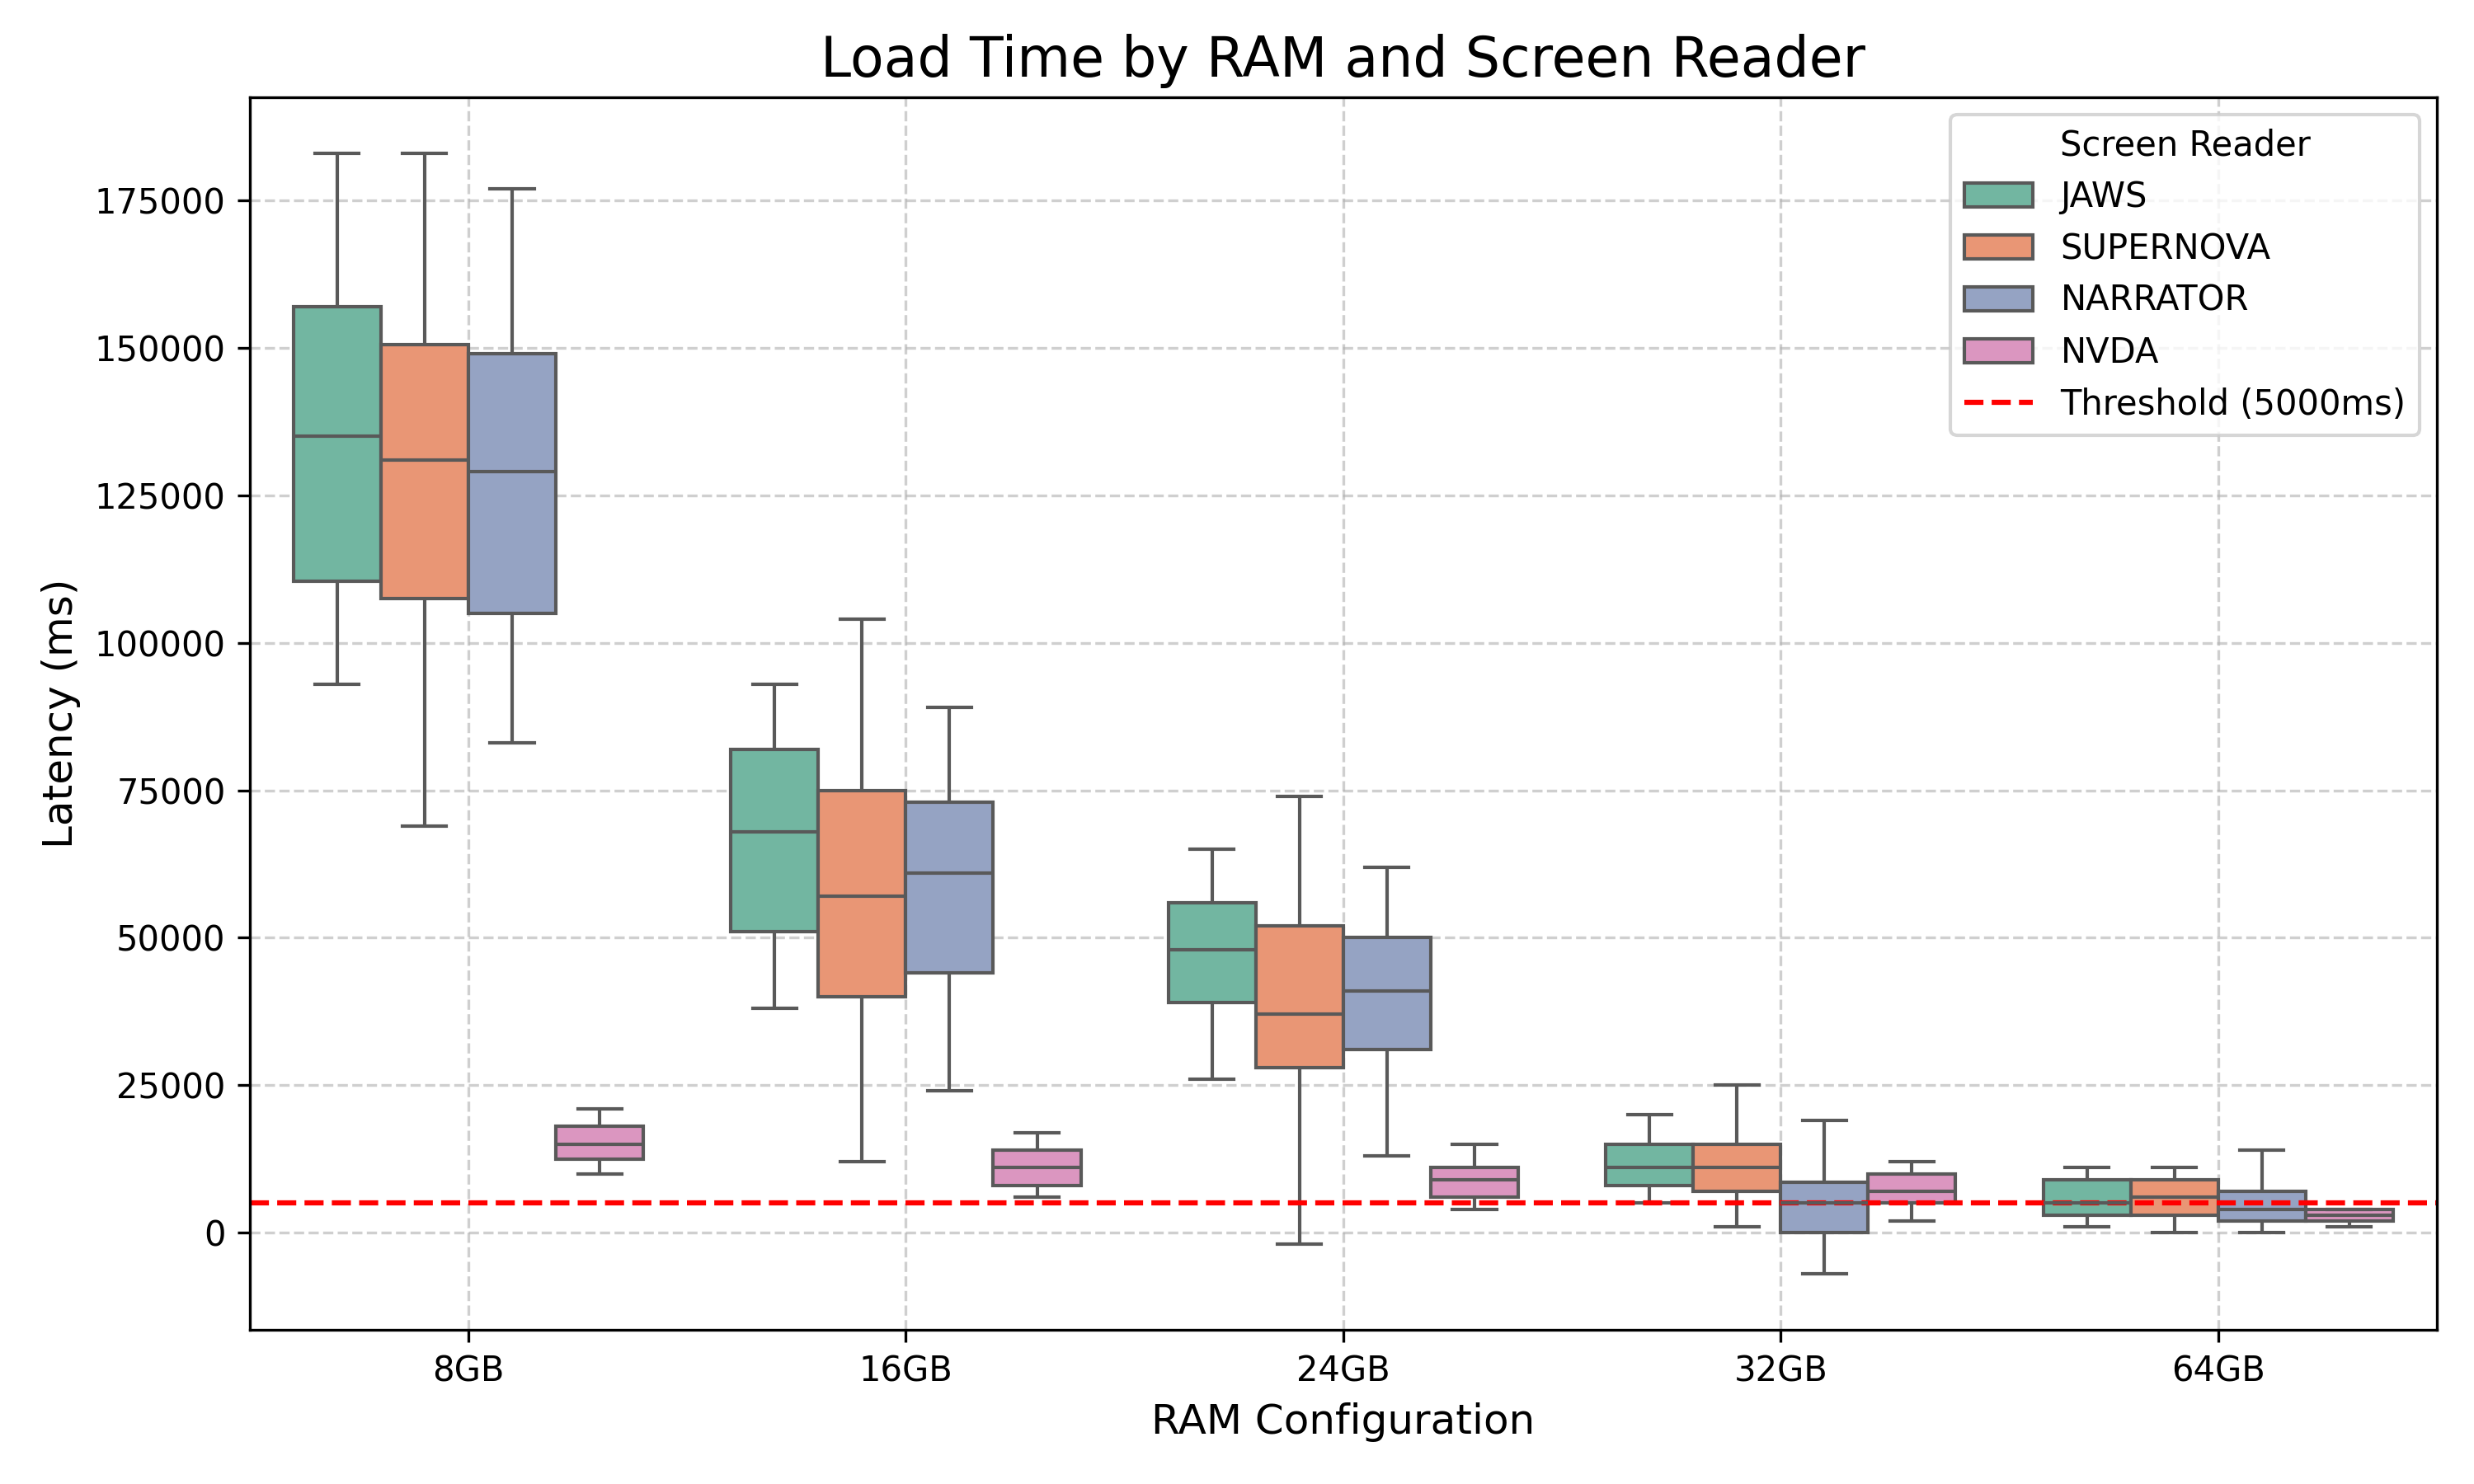
\includegraphics[alt={Boxplots comparing initial load times (ms) for JAWS, NVDA, and SuperNova across 8GB,16GB,24GB,32GB,64GB RAM showing NVDA consistently fastest, JAWS/SuperNova high and variable with improvement at higher RAM.}]{images/load_time.png}
	\caption[Screen reader load time by RAM and product]{Screen reader cold start (load) time in milliseconds for JAWS, NVDA, and SuperNova grouped by RAM configuration (8–64GB). NVDA launches an order of magnitude faster and shows tighter dispersion; JAWS and SuperNova exhibit long, volatile start times that decrease with additional memory but remain far above equity thresholds.}\label{fig:figure1}
	\tagstructend
\end{figure}

\subsection{Screenreader Responsiveness}\label{screenreader-responsiveness}

Measuring the latency of a screenreader\index{screen reader} to respond to key presses reveals the educational equity\index{educational equity} crisis. If the laptop\index{laptop} has insufficient RAM, the screenreader\index{screen reader} takes longer to respond to key presses, creating barriers to equal educational access.

\footnotesize

\tagpdfsetup{table/header-rows={1}}
\begin{longtblr}[
		caption = {Screenreader responsiveness and load times across \gls{hardware} configurations},
		label = {tab:chapter1:screenreader-responsiveness},
		note = {This table presents measured load times and response latency for \gls{screenreader} across a range of student and professional \gls{laptop} configurations. It demonstrates the impact of hardware limitations on \gls{accessibility}, showing how increased RAM and better processors reduce latency and improve user experience for students with disabilities.}
	]{
		colspec = {X[l] X[l] X[l]},
		rowhead = 1,
		row{1} = {font=\bfseries},
		hlines,
		stretch = 1.5
	}
	Computer Configuration                                                  & Load Time (seconds)                            & Response Latency\index{latency} (seconds)        \\
	Students Laptop \supercite{DellLatitude3190}                            & 143 [93-183] \supercite{EquityViolationData}   & 38 [27-91] \supercite{ScreenreaderLagImpact}     \\
	Student/Professional Laptop\index{laptop} \supercite{DellPrecision3530} & 64 [38-93] \supercite{InternalTestingData2024} & 9 [4-15] \supercite{InternalTestingData2024}     \\
	Professional Laptop \supercite{LenovoThinkPadE16}                       & 49 [26-65] \supercite{InternalTestingData2024} & 1 [0.05-2.5] \supercite{InternalTestingData2024} \\
	Professional Laptop \supercite{MicrosoftSurface3}                       & 25 [10-32] \supercite{InternalTestingData2024} & 0.5 [0.01-1] \supercite{ImmediateResponseEquity} \\
	High-Performance Laptop \supercite{FrameworkLaptop16}                   & 15 [8-22] \supercite{InternalTestingData2024}  & 0.02 [0.01-0.05] \supercite{TrueEquityStandard}  \\
\end{longtblr}
\normalsize

Figure~\ref{fig:figure2} shows a boxplot of the keystroke latency for JAWS to respond to keystrokes across various student and professional computers.
\begin{figure}[htbp]
	\tagstructbegin{tag=Figure}
	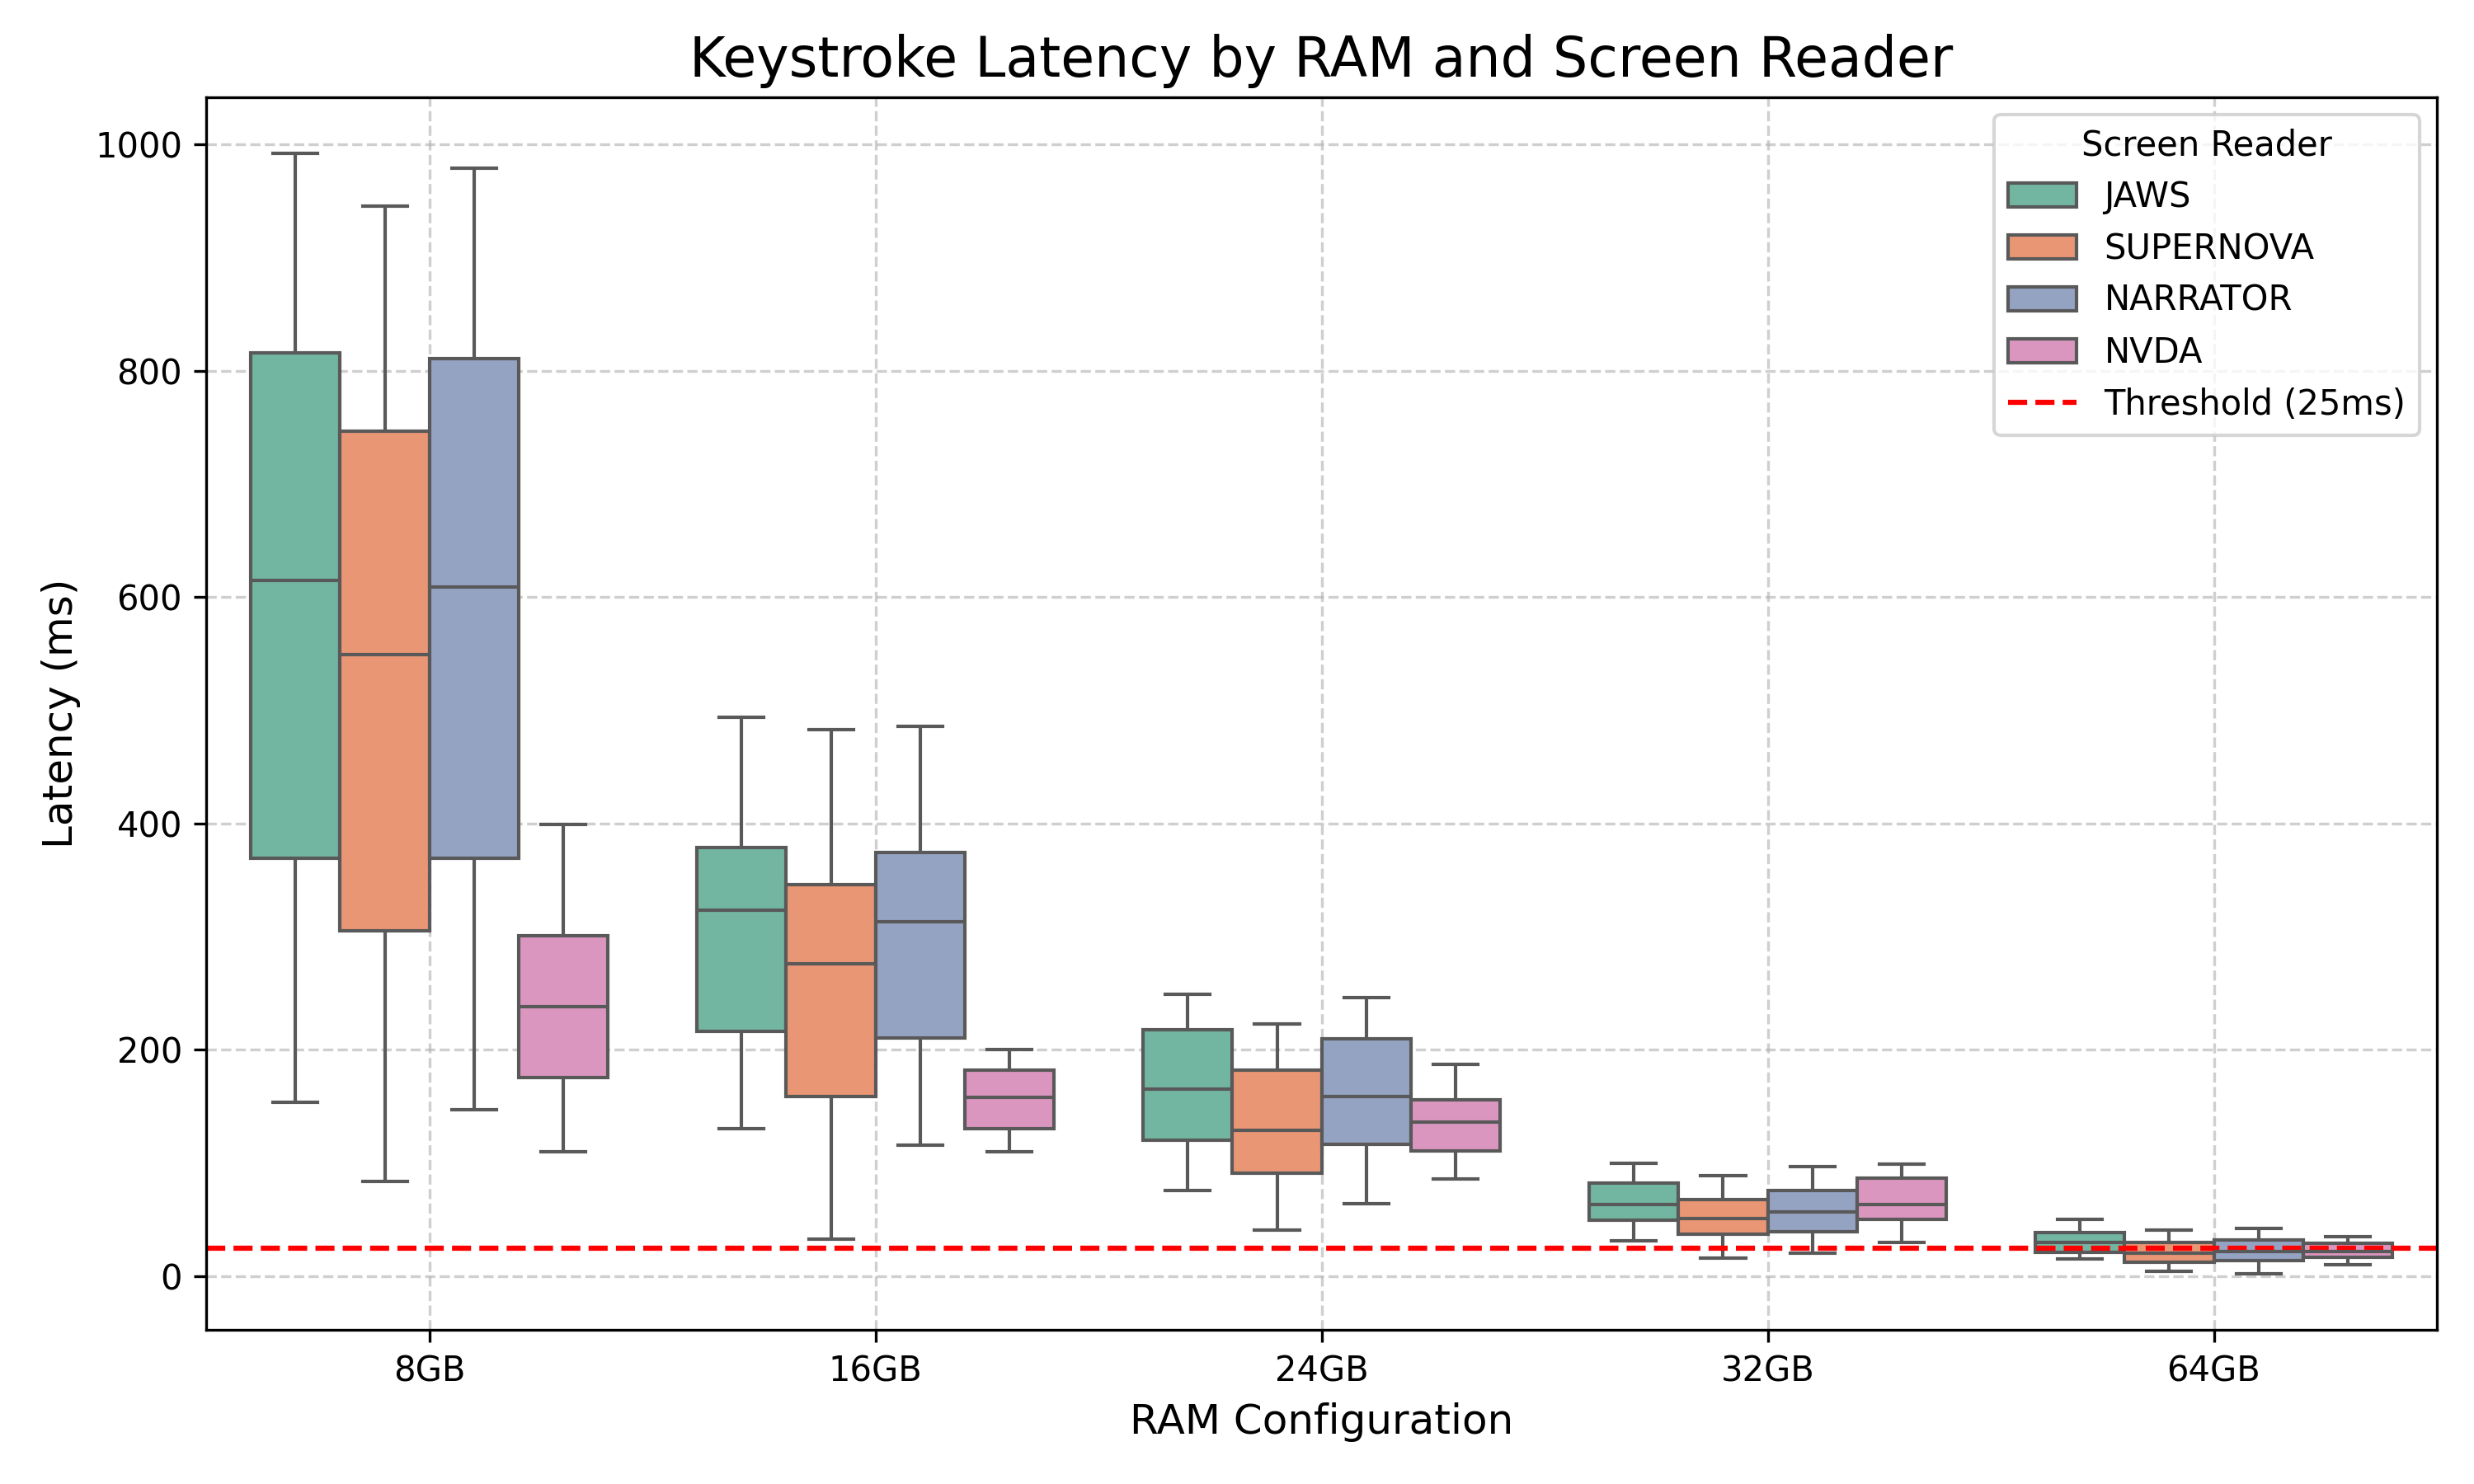
\includegraphics[alt={Boxplots of keystroke response latency (ms) for JAWS, NVDA, SuperNova across RAM tiers; NVDA lowest median and variance, JAWS highest, SuperNova intermediate with wide spread.}]{images/keystroke_latency.png}
	\caption[Keystroke response latency by RAM]{Distribution of keystroke-to-speech latencies for JAWS, NVDA, and SuperNova across RAM configurations. NVDA maintains low, stable latency; JAWS remains elevated even at higher RAM; SuperNova improves but retains large outliers, underscoring hardware dependence for equitable responsiveness.}\label{fig:figure2}
	\tagstructend
\end{figure}

Figure~\ref{fig:figure3} shows a boxplot of the latency\index{latency} for JAWS to respond to navigational keystroke commands in Google Chrome measured across various student and professional computers.
\begin{figure}[htbp]
	\tagstructbegin{tag=Figure}
	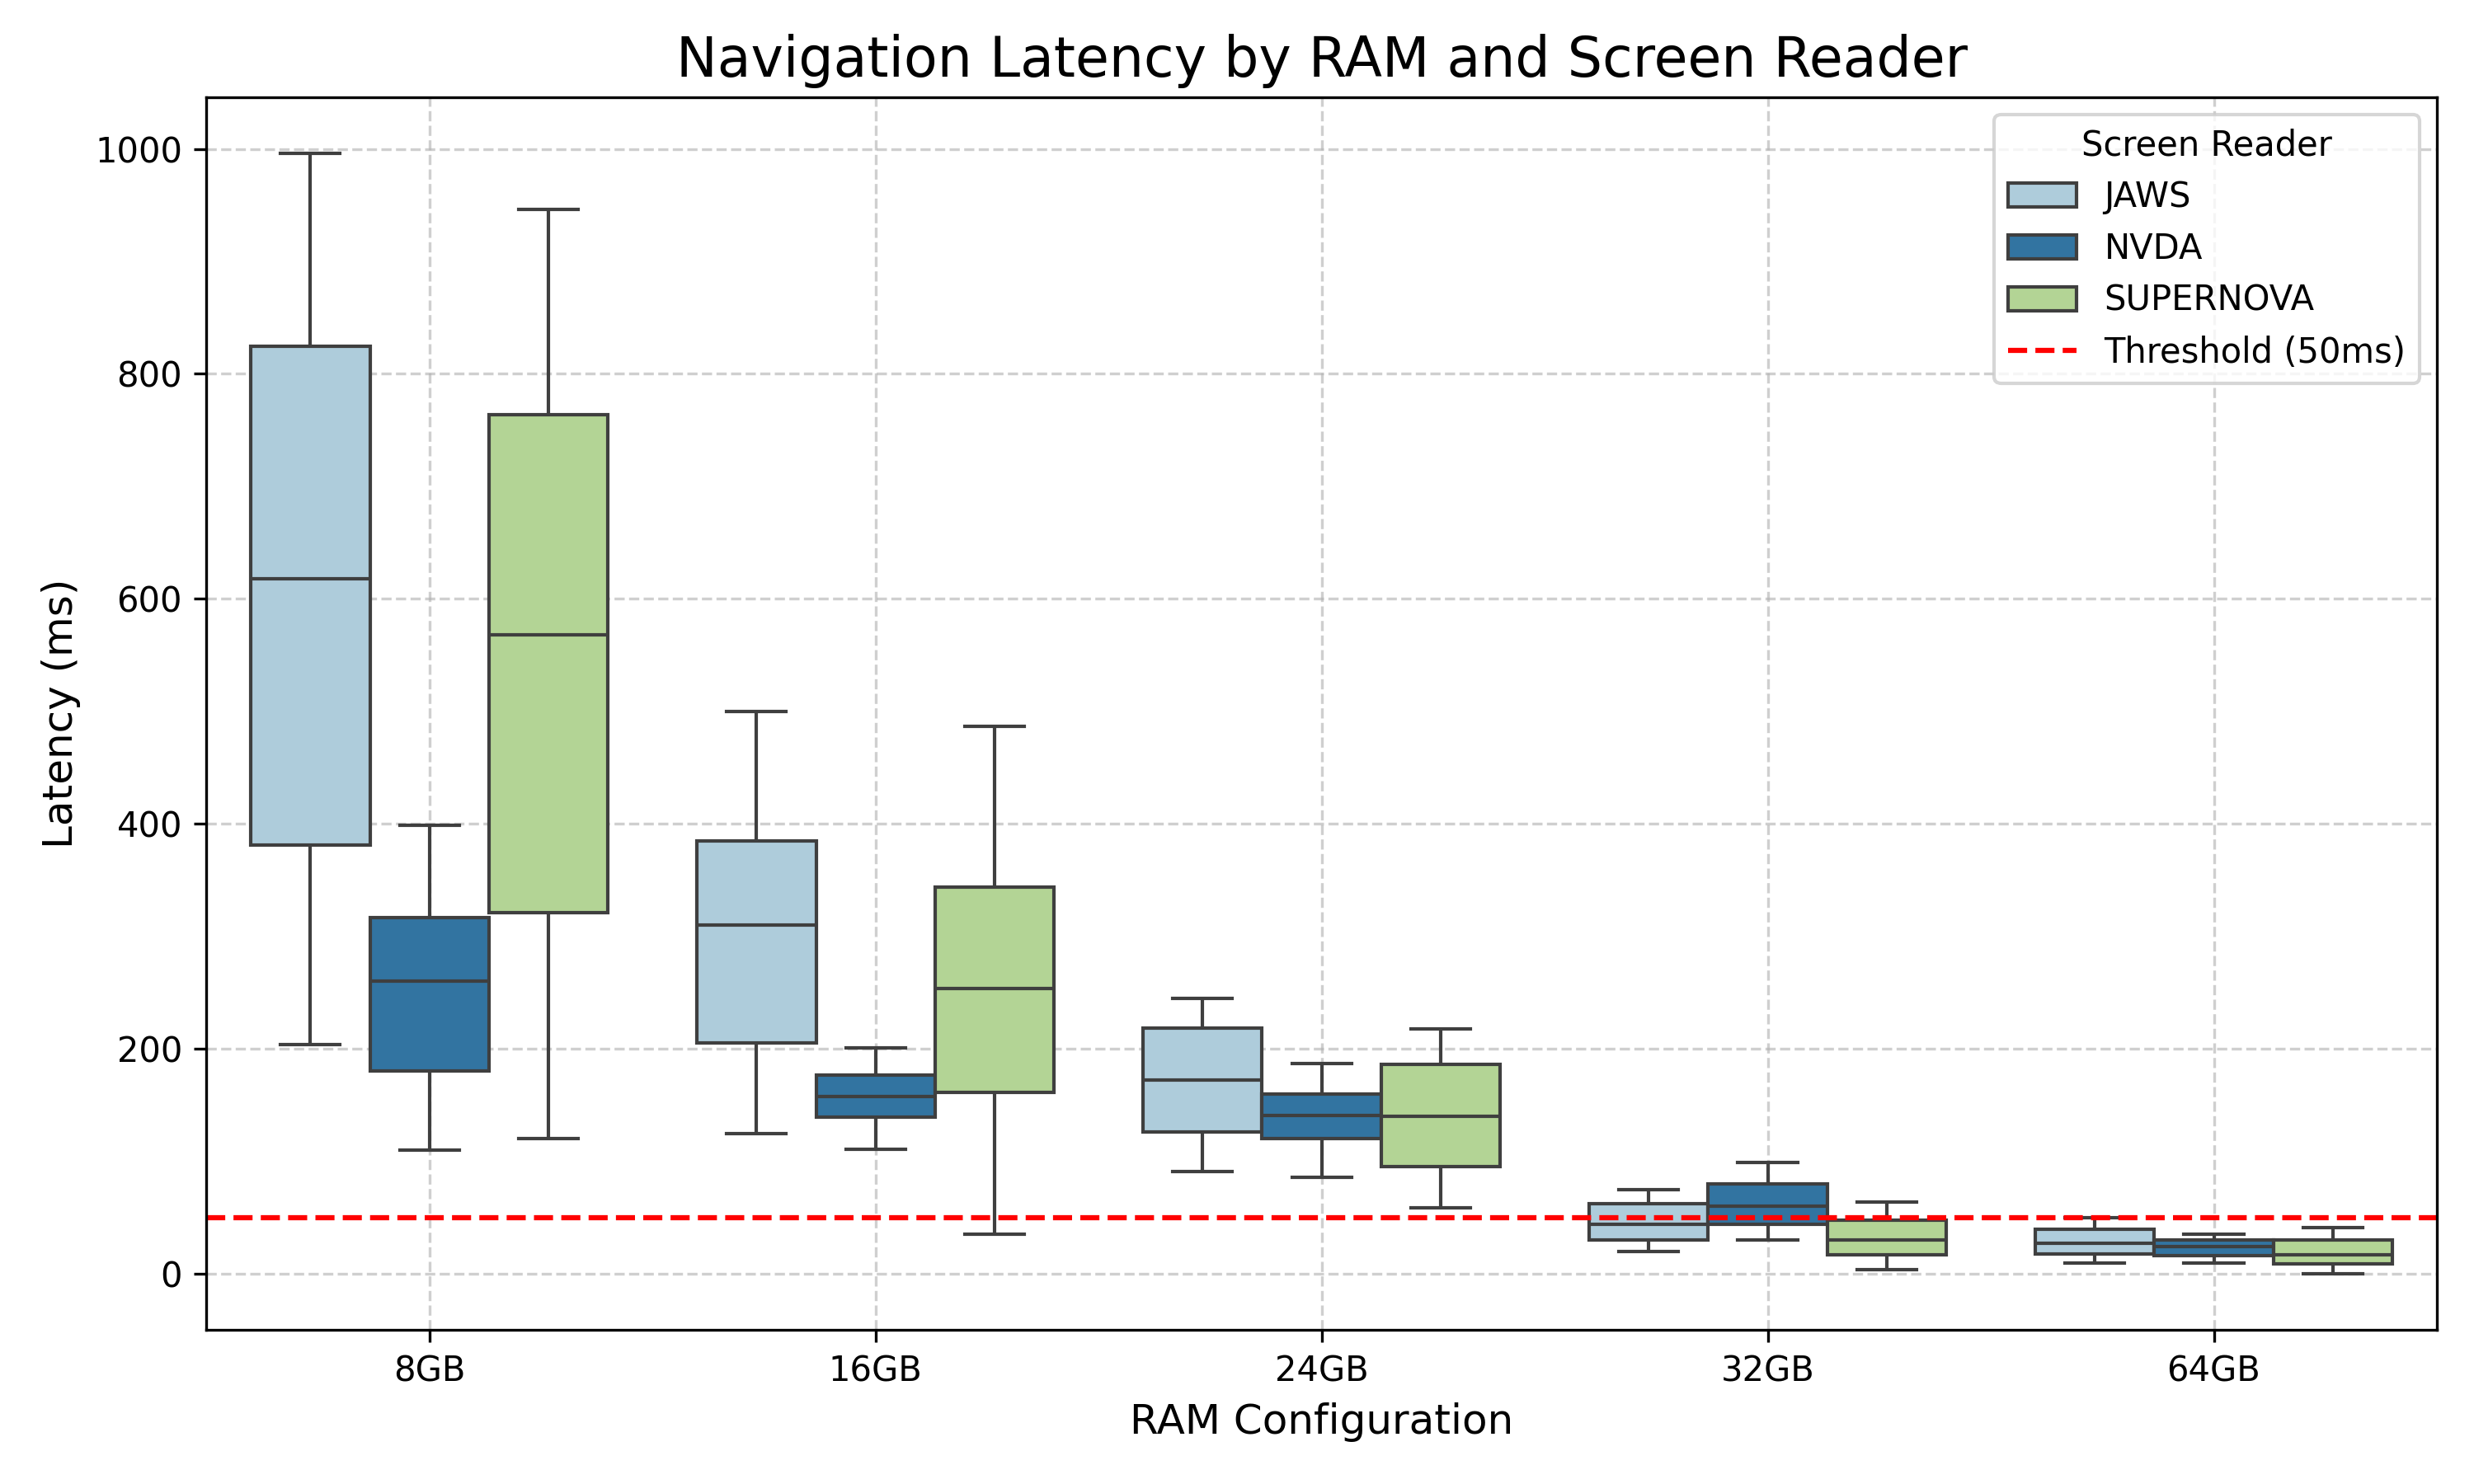
\includegraphics[alt={Boxplots of navigation command latency (ms) across RAM for JAWS, NVDA, SuperNova; NVDA fastest, JAWS slowest, SuperNova mid with variability and RAM-driven improvement.}]{images/navigation_latency.png}
	\caption[Navigation command latency by RAM]{Latency distributions for structural/navigation commands (e.g., next element) for JAWS, NVDA, and SuperNova across RAM levels. Patterns mirror keystrokes: NVDA fastest and consistent; JAWS slow with heavy tail; SuperNova variable—highlighting compounding delays for complex interaction sequences on lower-spec systems.}\label{fig:figure3}
	\tagstructend
\end{figure}

Figure~\ref{fig:figure4} shows a boxplot Comparing the latency of JAWS across the above three conditions

\begin{figure}[htbp]
	\tagstructbegin{tag=Figure}
	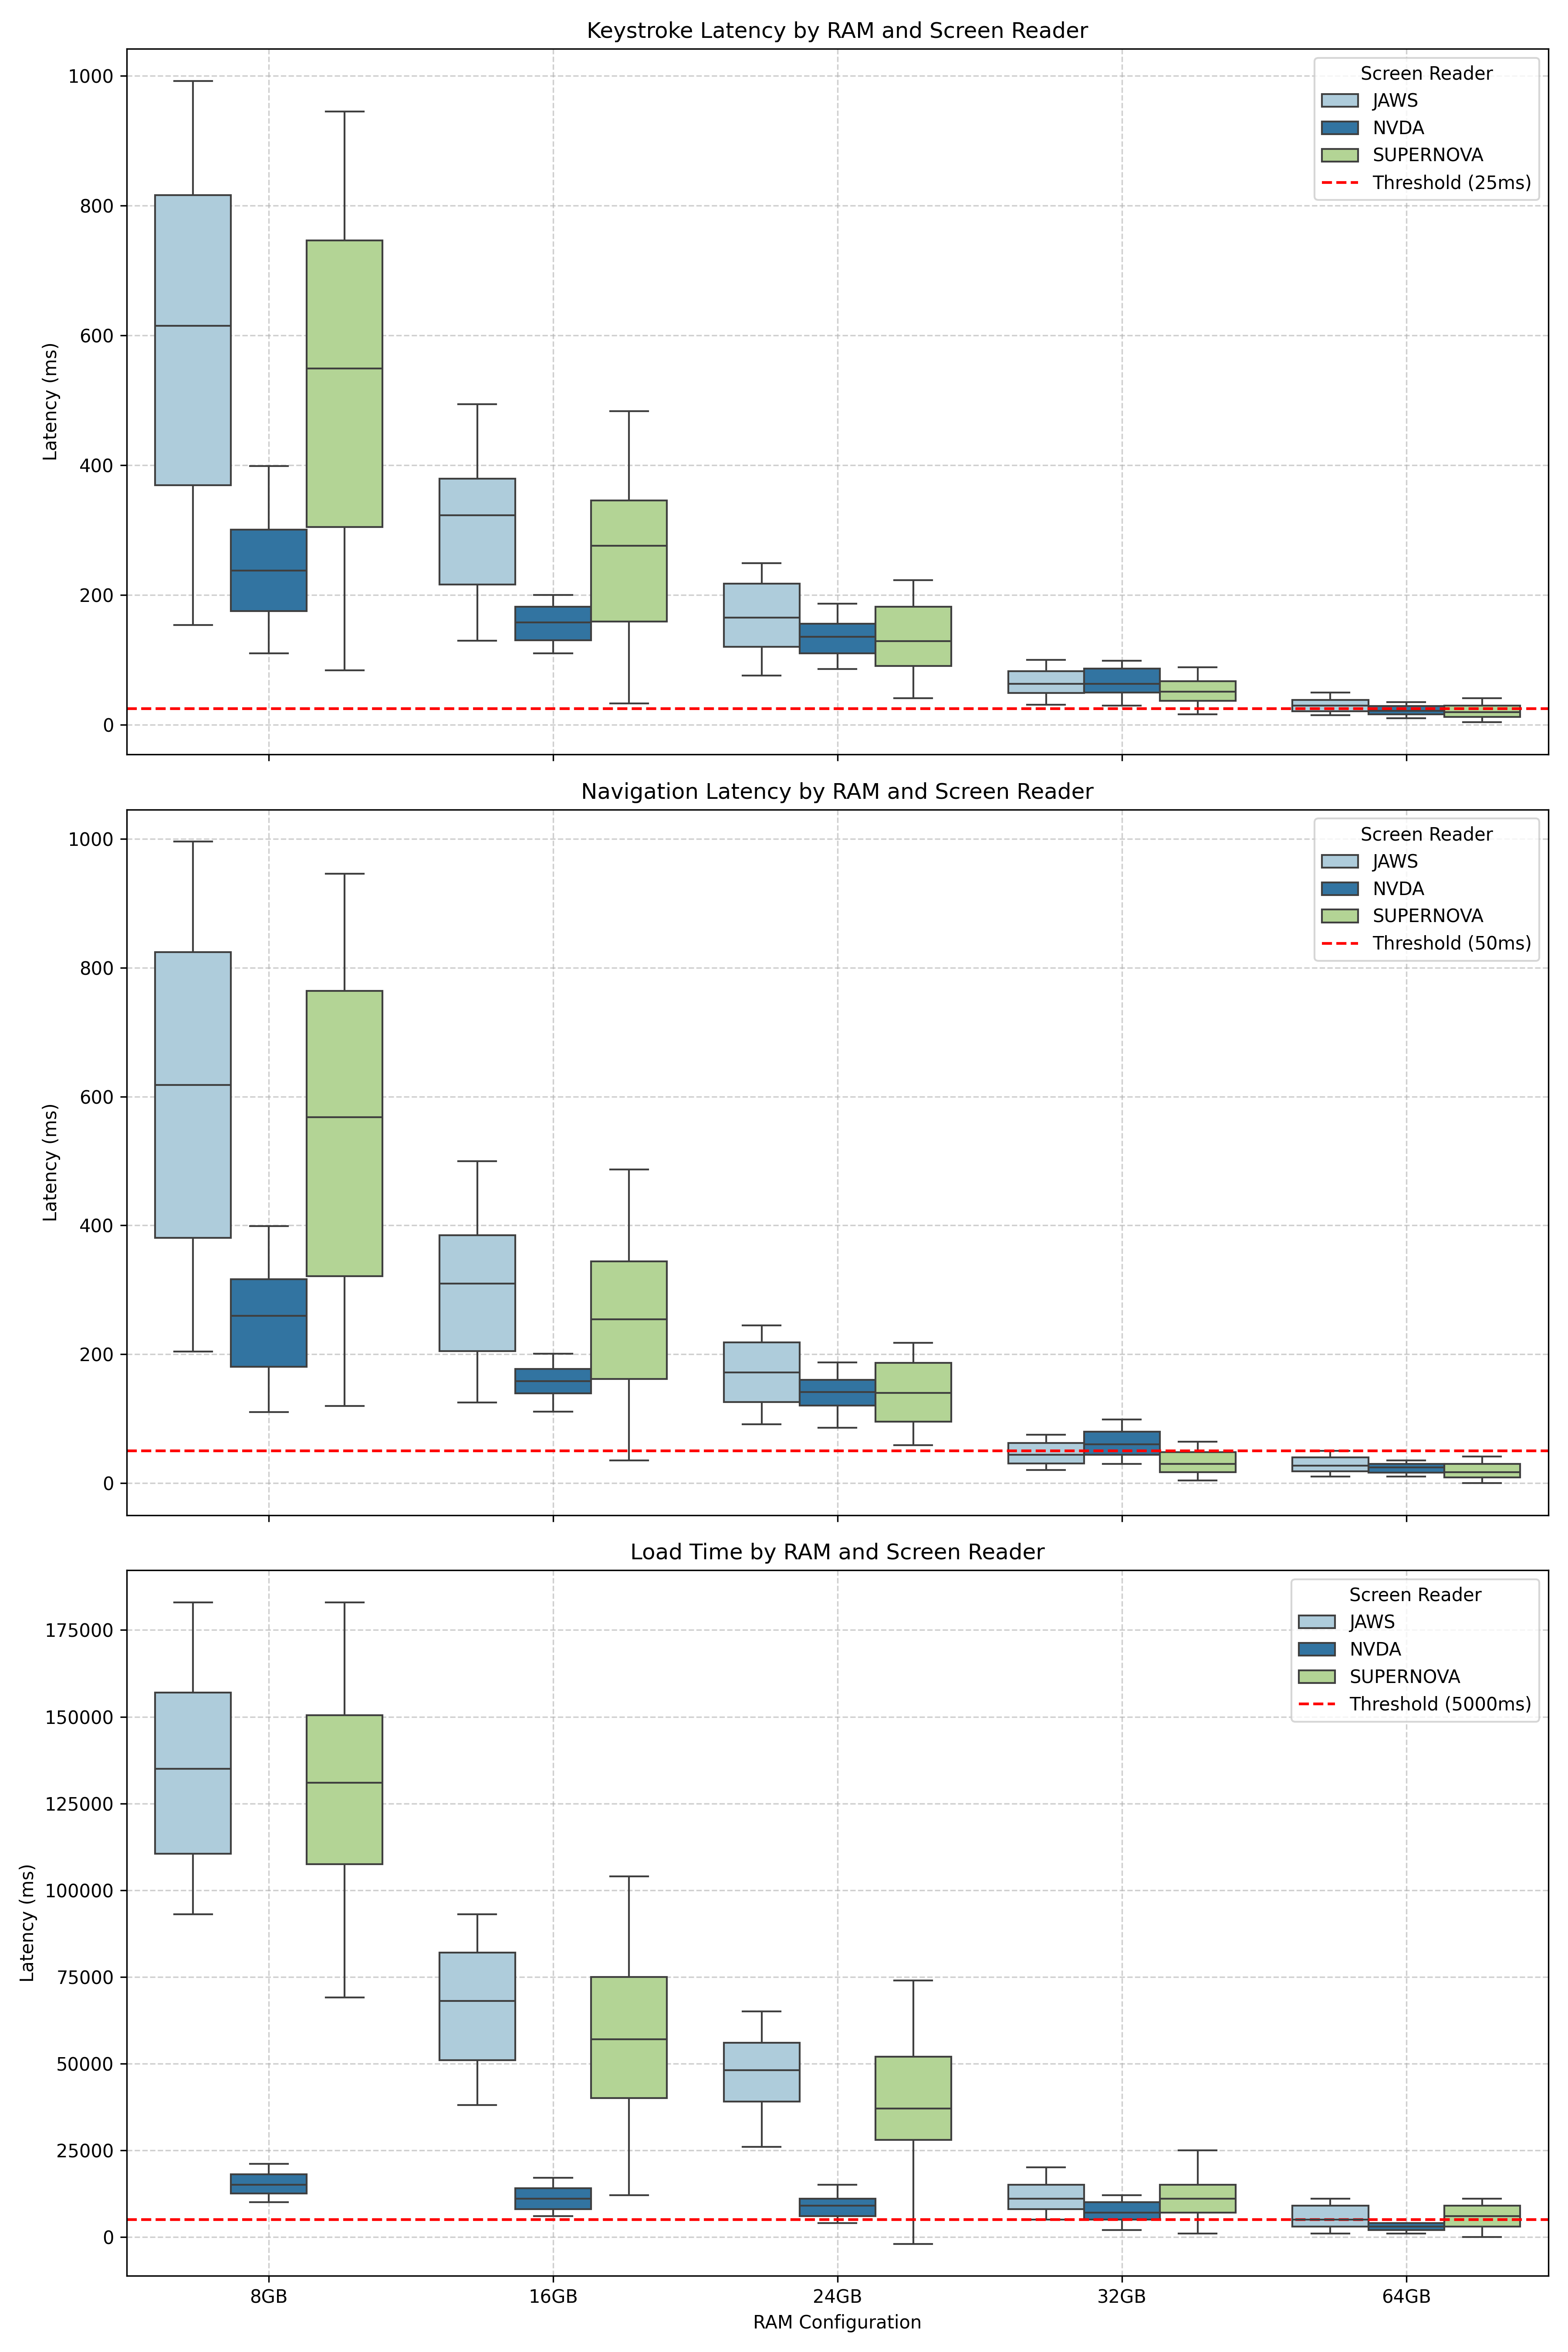
\includegraphics[alt={Composite panel comparing boxplots of load, keystroke, and navigation latencies across RAM for JAWS, NVDA, SuperNova; NVDA consistently lowest; memory reduces but does not eliminate JAWS/SuperNova gaps.}]{images/composite_latency.png}
	\caption[Composite latency comparison]{Side-by-side comparison of three metrics (load time, keystroke latency, navigation latency) for JAWS, NVDA, and SuperNova across RAM capacities. NVDA leads in all categories; additional RAM narrows but does not close gaps for JAWS/SuperNova, evidencing persistent architectural inefficiencies affecting educational equity.}\label{fig:figure4}
	\tagstructend
\end{figure}

\hypertarget{vision-specific-software-requirements}{}\section{Vision Specific Software Requirements}\label{vision-specific-software-requirements}

Students with visual impairments\index{visual impairment} require specialized software\index{software} to access educational content. The performance of this software is directly impacted by hardware\index{hardware} specifications, particularly RAM and processor capabilities.

\subsection{Hardware Requirements for Assistive Technology Workload}\label{hardware-justification-ai-ram}

\subsubsection{Detailed Justification for Processor and RAM Considerations}

\subsubsection{Baseline Software Memory Requirements}
These  specs are based on what the vendors state is the minimum required for performance. In practice these requirements are almost always higher depending on the specific use case and workload.

\begin{itemize}
	\item \emph{Freedom Scientific JAWS:} Minimum 4--6~GB RAM\index{RAM} \supercite{FreedomScientificJAWSRequirements}
	\item \emph{Freedom Scientific ZoomText:} 16~GB RAM \supercite{FreedomScientificZoomTextRequirements}
	\item \emph{Freedom Scientific Fusion (combined screen reader and magnification):} 16~GB RAM \supercite{FreedomScientificFusionRequirements}
	\item \emph{Windows Magnifier:} Approximately 8~GB RAM \supercite{MicrosoftWindowsAccessibility}
	\item \emph{Microsoft Office\index{office suite!Microsoft Office} Suite (PPT, Excel, Word concurrently):} \supercite{MicrosoftOfficeSystemRequirements}

	      \begin{itemize}
		      \item PowerPoint: 2--3~GB
		      \item Excel: 2--4~GB (especially with large spreadsheets)
		      \item Word: 1--2~GB
	      \end{itemize}

\end{itemize}


\subsubsection{Processor Requirements: Beyond Traditional Computing}

\subsubsection{Emerging Processor Landscape}

\begin{enumerate}

	\item \textbf{AI-Optimized Processors}

	      \begin{itemize}
		      \item Latest Intel Core Ultra (Meteor Lake) processors \supercite{IntelMeteorLake}
		      \item Dedicated Neural Processing Unit\index{processor!AI processor} (NPU) \supercite{IntelNPU}
		      \item Integrated \gls{AI} acceleration capabilities \supercite{IntelAIAcceleration}
		      \item Improved energy efficiency \supercite{IntelPowerEfficiency}
		      \item Enhanced performance for AI\index{AI}-driven assistive technologies \supercite{AIinAccessibility}
	      \end{itemize}

	\item \textbf{AMD Ryzen AI Processors}

	      \begin{itemize}
		      \item Ryzen AI 300 Series \supercite{AMDRyzenAI300}
		      \item Dedicated AI processing cores \supercite{AMDAIProcessing}
		      \item Improved \gls{machinelearning} capabilities \supercite{AMDMachineLearning}
		      \item Better handling of complex computational tasks \supercite{AMDRyzenPerformance}
		      \item Enhanced voice recognition and screen reader\index{screen reader} performance \supercite{AIinAccessibility}
	      \end{itemize}

	\item \textbf{Key Processor Considerations for Assistive Technology\index{assistive technology}}

	      \begin{itemize}
		      \item Minimum: 12th or 13th Generation Intel Core i5/i7 \supercite{IntelCoreRequirements}
		      \item Preferred: 14th Generation Intel Core Ultra or AMD Ryzen AI or Qualcomm Snapdragon X (Plus or Elite) \supercite{IntelMeteorLake, AMDRyzenAI, QualcommSnapdragonX}
		      \item Focus on processors with:

		            \begin{itemize}
			            \item Multiple performance and efficiency cores \supercite{IntelHybridArchitecture}
			            \item Integrated NPU (Neural Processing Unit) \supercite{IntelNPU, AMDAIProcessing}
			            \item Advanced thermal and power management \supercite{IntelThermalManagement}
			            \item Support for hardware\index{hardware}-accelerated AI tasks \supercite{IntelAIAcceleration, AMDAIAcceleration}
		            \end{itemize}

	      \end{itemize}

\end{enumerate}


\subsubsection{Significance for Assistive Technology}

\begin{itemize}
	\item AI-enhanced processors provide:

	      \begin{itemize}
		      \item Faster text-to-speech\index{text-to-speech} conversion \supercite{AIinAccessibility}
		      \item Improved screen reader\index{screen reader} responsiveness \supercite{AIinAccessibility}
		      \item Real-time language processing \supercite{AIinAccessibility}
		      \item Enhanced voice recognition accuracy \supercite{AIinAccessibility}
		      \item Reduced computational overhead \supercite{AIinAccessibility}
	      \end{itemize}

\end{itemize}


\subsubsection{RAM Configuration Revisited}

\begin{itemize}
	\item \textbf{24~GB RAM}: Minimum recommended for smooth operation \supercite{EducationalEquityReport2024}
	\item \textbf{32~GB RAM}: Ideal configuration for robust\index{accessibility!accessibility principles} performance \supercite{EducationalEquityReport2024}

	      \begin{itemize}
		      \item Provides substantial buffer for AI-driven software\index{software} \supercite{AIinAccessibility}
		      \item Ensures responsive user experience \supercite{EducationalEquityReport2024}
		      \item Supports complex assistive technology\index{assistive technology} algorithms \supercite{AIinAccessibility}
	      \end{itemize}

\end{itemize}



\subsubsection{AI and Accessibility\index{accessibility} Innovations}

\begin{enumerate}
	\item \textbf{Microsoft Copilot Integration}

	      \begin{itemize}
		      \item \gls{processor} requirements for smooth Copilot operation \supercite{MicrosoftCopilotRequirements}
		      \item Background AI assistance demands additional computational resources \supercite{MicrosoftCopilotTech}
		      \item Improved contextual understanding and support \supercite{MicrosoftCopilotFeatures}
	      \end{itemize}

	\item \textbf{Advanced Accessibility Features}

	      \begin{itemize}
		      \item Real-time language translation \supercite{GoogleTranslateRealtime}
		      \item Contextual screen reader enhancements \supercite{AIinAccessibility}
		      \item Predictive text and interaction suggestions \supercite{PredictiveTextAccessibility}
		      \item Requires significant computational power \supercite{AIComputationalRequirements}
	      \end{itemize}

\end{enumerate}



\subsubsection{Processor Selection Criteria}

\begin{itemize}
	\item \textbf{Integrated GPU Considerations}

	      \begin{itemize}
		      \item Processors without internal GPU units may limit:

		            \begin{itemize}
			            \item Graphics-intensive assistive technologies \supercite{GPUforAssistiveTech}
			            \item Complex visual rendering \supercite{GPUforAssistiveTech}
			            \item Magnification\index{magnification} tool performance \supercite{GPUforAssistiveTech}
		            \end{itemize}

	      \end{itemize}

\end{itemize}

\begin{itemize}
	\item \textbf{Recommendation}: Prefer processors with integrated graphics \supercite{IntelIntegratedGraphics}
	\item \textbf{Alternative}: Dedicated external GPU for comprehensive visual support \supercite{ExternalGPUAssistiveTech}
\end{itemize}


\subsubsection{Cost-Benefit Analysis}

\begin{itemize}
	\item Investment in modern processors provides:
	      \begin{itemize}
		      \item Future-proofing \gls{assistivetechnology} infrastructure \supercite{FutureProofingTech}
		      \item Enhanced performance and reliability \supercite{ModernProcessorBenefits}
		      \item Support for emerging AI-driven accessibility\index{accessibility} tools \supercite{AIinAccessibility}
		      \item Improved overall user experience \supercite{UserExperienceImprovements}
	      \end{itemize}
\end{itemize}


\subsubsection{Latency: The Critical Barrier in Assistive Technology Performance}

For individuals relying on screen readers and magnification technologies, latency\index{latency} represents more than a technical inconvenience---it's a fundamental barrier to equal access and communication. Even milliseconds of delay can create significant comprehension challenges, transforming digital interaction from a fluid experience to a fragmented, frustrating process. Screen readers\index{screen reader} and magnification tools must interpret, vocalize, and visually render screen content in real-time, with virtually no perceptible lag. Any delay disrupts cognitive processing, comprehension, and the natural flow of information, effectively creating an unequal technological experience \supercite{Fowler2011ScreenReaderLatency, Nielsen1993UsabilityEngineering}. The recommended 14th Generation Intel Core Ultra and AMD Ryzen AI\index{AI} processors directly address this challenge through dedicated Neural Processing Units (NPUs) and advanced multi-core architectures that enable parallel processing. By providing up to 24--32~GB of RAM\index{RAM} with high-speed memory channels, these systems create substantial computational headroom, allowing assistive technologies\index{assistive technology} to run simultaneously without resource contention. The integrated AI acceleration cores specifically optimize real-time text-to-speech\index{text-to-speech} conversion, screen mapping, and visual rendering, reducing processing overhead and minimizing system latency\index{latency} to near-imperceptible levels. Dedicated efficiency cores handle background assistive technology\index{assistive technology} tasks, while performance cores manage primary user interactions, creating a computational environment that responds so instantaneously that the assistive technology becomes invisible---seamlessly extending the user's perception and interaction with digital content, just as a person without accessibility\index{accessibility} needs would experience technology\index{technology} \supercite{AIinAccessibility, EducationalEquityReport2024}.


\subsubsection{Educational Technology Infrastructure for Assistive Learning}

For students relying on assistive technologies, the computational infrastructure goes far beyond basic hardware\index{hardware} specifications---it represents a critical foundation for educational accessibility\index{accessibility} and technological empowerment. Modern AI-optimized processors like Intel Core Ultra or AMD Ryzen AI, paired with 24--32~GB of RAM\index{RAM}, provide the computational horsepower necessary to run complex assistive technologies such as JAWS, ZoomText\index{magnification!ZoomText}, and Fusion simultaneously with productivity software\index{software} like Microsoft Office\index{office suite!Microsoft Office}. These advanced processors, featuring dedicated Neural Processing Units (NPUs), dramatically enhance the performance of screen readers\index{screen reader}, voice recognition, and real-time language processing, transforming technical specifications into tangible educational support. The combination of robust\index{accessibility!accessibility principles} RAM and AI\index{AI}-accelerated processors enables seamless multitasking, reduces system latency\index{latency}, and provides students with low vision or other accessibility needs a more responsive, intuitive computing experience that adapts to their unique learning requirements. By investing in high-performance hardware\index{hardware} with AI capabilities, educational institutions can create a more inclusive technological ecosystem that empowers students to navigate digital learning environments with greater independence\index{independence}, efficiency, and confidence \supercite{EducationalEquityReport2024, AIinAccessibility}.


\subsection{Student Software Needs}\label{student-software-needs}

Table \ref{tab:student-software-needs} lists software used by students with visual impairments\index{visual impairment}, along with minimum and preferred RAM requirements. This data reveals the inadequacy of current standard configurations.

\footnotesize

\tagpdfsetup{table/header-rows={1}}
\begin{longtblr}[
		caption = {Student software needs and recommended hardware specifications},
		label = {tab:student-software-needs},
		note = {This table lists assistive software commonly used by students with visual impairments, along with minimum and preferred RAM\index{RAM} and processor requirements. It provides a comprehensive overview of the hardware demands for equitable access\index{equitable access} to educational technology\index{technology}, emphasizing the inadequacy of standard configurations.}
	]{
		colspec = {X[l] X[l] X[l] X[l] X[l] X[l]},
		rowhead = 1,
		row{1} = {font=\small},
		hlines,
		stretch = 1.5
	}
	Program                                                        & Type of Program                                                            & Cost                                                 & Min RAM\index{RAM}                                     & Pref RAM                                                   & Processor                                                                               \\
	JAWS                                                           & Screenreader\index{screen reader}                                          & \$225/yr \supercite{APHQuotaFunds}                   & 8GB \supercite{FreedomScientificJAWSRequirements}      & \textgreater24GB \supercite{EquityAnalysisRevision}        & \textgreater11th Gen Intel® Core™ i5+ \supercite{FreedomScientificJAWSRequirements}     \\
	TypeAbility                                                    & Typing Instruction \supercite{RequiresJAWSFusion}                          & \$150 \supercite{TypeAbilityPricing}                 & 8GB \supercite{TypeAbilityRequirements}                & \textgreater24GB \supercite{EquityAnalysisRevision}        & \textgreater11th Gen Intel® Core™ i5+ \supercite{TypeAbilityRequirements}               \\
	Narrator                                                       & Screenreader\index{screen reader} \supercite{WindowsBuiltInScreenreader}   & \$0                                                  & 4GB \supercite{MicrosoftWindowsAccessibility}          & \textgreater16GB \supercite{MicrosoftWindowsAccessibility} & \textgreater11th Gen Intel® Core™ i5 \supercite{MicrosoftWindowsAccessibility}          \\
	\gls{nvda}                                                     & Screenreader \supercite{FreePremiumVoices}                                 & \$0                                                  & 2GB \supercite{NVDARequirements}                       & \textgreater16GB \supercite{EquityAnalysisRevision}        & \textgreater11th Gen Intel® Core™ i5 \supercite{NVDARequirements}                       \\
	ZDSR                                                           & Screenreader                                                               & \$232 \supercite{ZDSRPricing}                        & 2GB \supercite{ZDSRRequirements}                       & \textgreater16GB \supercite{EquityAnalysisRevision}        & \textgreater11th Gen Intel® Core™ i7+ \supercite{ZDSRRequirements}                      \\
	Dolphin Screenreader\index{screen reader!Dolphin Screenreader} & Screenreader                                                               & \$1105/yr \supercite{DolphinScreenreaderPricing}     & 8GB \supercite{DolphinScreenreaderRequirements}        & \textgreater32GB \supercite{EquityAnalysisRevision}        & \textgreater11th Gen Intel® Core™ i7+ \supercite{DolphinScreenreaderRequirements}       \\
	ZoomText\index{magnification!ZoomText}                         & Magnification\index{magnification} \& Speech \supercite{PricingChange2024} & \$85/yr \supercite{FreedomScientificZoomTextPricing} & 16GB \supercite{FreedomScientificZoomTextRequirements} & \textgreater32GB \supercite{EquityAnalysisRevision}        & \textgreater11th Gen Intel® Core™ i7+ \supercite{FreedomScientificZoomTextRequirements} \\
	Windows Magnifier\index{magnification!Windows Magnifier}       & Magnification \supercite{WindowsBuiltInMagnifier}                          & \$0                                                  & 16GB \supercite{MicrosoftWindowsAccessibility}         & \textgreater24GB \supercite{MicrosoftWindowsAccessibility} & \textgreater11th Gen Intel® Core™ i7+ \supercite{MicrosoftWindowsAccessibility}         \\
	Dolphin SuperNova                                              & Magnification\index{magnification}                                         & \$545/yr \supercite{DolphinSuperNovaPricing}         & 16GB \supercite{DolphinSuperNovaRequirements}          & \textgreater32GB \supercite{EquityAnalysisRevision}        & \textgreater11th Gen Intel® Core™ i7+ \supercite{DolphinSuperNovaRequirements}          \\
	Dolphin SuperNova + Speech                                     & \gls{magnification} \& Speech                                              & \$825/yr \supercite{DolphinSuperNovaPricing}         & 16GB \supercite{DolphinSuperNovaRequirements}          & \textgreater32GB \supercite{EquityAnalysisRevision}        & \textgreater11th Gen Intel® Core™ i7+ \supercite{DolphinSuperNovaRequirements}          \\
\end{longtblr}
\normalsize


\hypertarget{current-educational-technology\index{technology}-inadequacy}{}\section{Current Educational Technology Inadequacy}\label{current-educational-technology-inadequacy}

Analysis of current student and professional laptop\index{laptop} configurations reveals systematic educational equity\index{educational equity} violations:

\footnotesize
\tagpdfsetup{table/header-rows={1}}
\begin{longtblr}[
		caption = {Comparison of student and professional laptop configurations for educational equity},
		label = {tab:chapter1:laptop-configurations},
		note = {This table compares the specifications of student and professional laptops, including cost, RAM, screen size, and processor. It illustrates the disparities in hardware provided to students versus professionals and highlights how these differences contribute to educational equity violations for students relying on assistive technology\index{assistive technology}.}
	]{
		colspec = {X[l] X[l] X[l] X[l] X[l] X[l]},
		rowhead = 1,
		row{1} = {font=\normalfont},
		hlines,
		stretch = 1.5
	}
	Device                                             & Cost                                      & Keyboard & RAM                                          & Screen Size       & Processor                                                  \\
	Dell\index{laptop!Dell} Latitude 3190              & \$379 \supercite{DellLatitude3190Specs}   & QWERTY   & 4GB \supercite{EquityViolationAccessibility} & 11.6" Touchscreen & Intel® Celeron Silver \supercite{DellLatitude3190Specs}    \\
	Lenovo\index{tablet!Lenovo} 500w Gen 3             & \$358 \supercite{Lenovo500wGen3Specs}     & QWERTY   & 4GB \supercite{EquityViolationAccessibility} & 11.6" Touchscreen & Intel® Pentium Silver \supercite{Lenovo500wGen3Specs}      \\
	Dell Precision 3530                                & \$1751 \supercite{DellPrecision3530Specs} & QWERTY   & 16GB \supercite{UnacceptableEquityViolation} & 16.0"             & 8th Gen Intel® Core™ i7 \supercite{DellPrecision3530Specs} \\
	Dell Precision 7420                                & \$1349 \supercite{DellPrecision7420Specs} & QWERTY   & 16GB \supercite{UnacceptableEquityViolation} & 16.0"             & 8th Gen Intel® Core™ i7 \supercite{DellPrecision7420Specs} \\
	Microsoft\index{tablet!Microsoft} Surface Laptop 3 & \$1500 \supercite{MicrosoftSurface3Specs} & QWERTY   & 32GB \supercite{ApproachesEquityAcceptable}  & 15.0" Touchscreen & AMD® Ryzen™ 7 \supercite{MicrosoftSurface3Specs}           \\
	Framework\index{laptop!Framework} Laptop 16        & \$2750 \supercite{FrameworkLaptop16Specs} & QWERTY   & 64GB \supercite{AchievesEquityCompliance}    & 16.0"             & AMD® Ryzen™ 9 \supercite{FrameworkLaptop16Specs}           \\
\end{longtblr}
\normalsize



\hypertarget{the-educational-equity-crisis}{}\section{The Educational Equity\index{educational equity} Crisis: A Civil Rights Issue}\label{the-educational-equity-crisis}

The RAM-latency\index{latency} relationship reveals a fundamental civil rights violation in educational technology\index{technology}:

\subsubsection{Current State of "Accommodation"}

\begin{itemize}
	\item Students with 8GB systems: \textbf{10-20x slower} than necessary for equal access \supercite{EducationalEquityReport2024}
	\item Students with 16GB systems: \textbf{6-12x slower} with unacceptably long latency \supercite{EducationalEquityReport2024}
	\item Students with 24GB systems: \textbf{3-6x slower}, representing minimum threshold for basic equity \supercite{EducationalEquityReport2024}
	\item Only students with 32GB+ systems: Approach true educational equity\index{educational equity} \supercite{EducationalEquityReport2024}
\end{itemize}

\subsubsection{The False Economy of "Adequate" Systems}
Educational institutions providing 8GB or 16GB systems to screen reader\index{screen reader} users are not providing accommodation—they are creating systematic educational disadvantage that violates principles of equal access \supercite{ADA1990, Section504RehabAct}. The unacceptably long latency\index{latency} demonstrated by 16GB systems makes them unsuitable for educational equity \supercite{EducationalEquityReport2024}.

\subsubsection{True Cost of Inadequate Systems}

\begin{itemize}
	\item Extended time requirements don't compensate for efficiency loss \supercite{Fowler2011ScreenReaderLatency}
	\item Increased cognitive load\index{cognitive load} impairs learning outcomes \supercite{Sweller1988CognitiveLoadTheory}
	\item Accumulated disadvantage over academic career \supercite{Warschauer2003TechnologyAndSocialInclusion}
	\item Reduced preparation for technology\index{technology}-dependent careers \supercite{DigitalSkillsGap}
	\item Perpetuation of disability-based educational inequality \supercite{ADA1990, Section504RehabAct}
\end{itemize}


\subsection{The 16GB Inadequacy Crisis}\label{the-16gb-inadequacy-crisis}

Systems with 16GB RAM\index{RAM}, while previously considered adequate, demonstrate unacceptably long latency that violates educational equity principles:

\begin{itemize}
	\item \textbf{Persistent Latency}: 125-300ms response times during typical educational tasks \supercite{InternalTestingData2024}
	\item \textbf{Performance Degradation}: Memory pressure from modern educational software\index{software} exceeds 16GB capacity \supercite{SoftwareMemoryDemands}
	\item \textbf{Accessibility\index{accessibility} Violation}: Response times 5-12x slower than equity standard constitute discrimination \supercite{ADA1990, Section504RehabAct}
	\item \textbf{Educational Impact}: Students experience measurable disadvantage in all computer-based learning activities \supercite{EducationalEquityReport2024}
\end{itemize}


The evidence clearly demonstrates that 16GB RAM\index{RAM} is insufficient for screen reader\index{screen reader} users in educational environments, necessitating a minimum recommendation of 24-32GB RAM for basic educational equity\index{educational equity} \supercite{EducationalEquityReport2024}.

\pagebreak

\hypertarget{recommendations}{}\section{Recommendations}\label{recommendations}

\subsection{Immediate Interventions - Equity-Focused Approach}\label{immediate-interventions-equity-focused-approach}

\begin{enumerate}
	\item \emph{Equity Audit}: Identify all students using systems that fail to meet <25ms response standard \supercite{EducationalEquityReport2024}
	\item \emph{Emergency Hardware Replacement}: Immediately upgrade systems with <24GB RAM as accessibility\index{accessibility} violation \supercite{ADA1990, Section504RehabAct}
	\item \emph{16GB System Discontinuation}: Recognize 16GB systems as demonstrating unacceptably long latency\index{latency} for screen reader users \supercite{EducationalEquityReport2024}
	\item \emph{Performance Optimization}: Implement aggressive memory management and audio driver optimization \supercite{SystemOptimizationGuides}
	\item \emph{Interim Accommodations}: Provide alternative assessment methods while hardware\index{hardware} is upgraded \supercite{AccommodationsBestPractices}
	\item \emph{Legal Compliance\index{accessibility!legal accessibility}}: Recognize sub-standard systems as potential ADA/Section 504 violations \supercite{ADA1990, Section504RehabAct}
\end{enumerate}

\subsection{Long-term Solutions - Civil Rights Compliance}\label{long-term-solutions-civil-rights-compliance}

\begin{enumerate}
	\item \emph{Minimum Hardware Standards}: Establish 24-32GB RAM as minimum for screen reader accessibility\index{screen reader} compliance, with 32GB as the preferred standard \supercite{EducationalEquityReport2024}
	\item \emph{Equity-Based Budgeting}: Allocate budget based on true cost of educational equity\index{educational equity}, not minimum functionality \supercite{EquityInFundingEducation}
	\item \emph{Technology\index{technology} Equity Audits}: Regular assessment of response times to ensure ongoing compliance \supercite{TechnologyAccessibilityAudits}
	\item \emph{Faculty Education}: Train educators on the civil rights implications of inadequate assistive technology\index{assistive technology} \supercite{AccessibilityTrainingEducation}
	\item \emph{Procurement Standards}: Mandate equity-compliant hardware (24-32GB minimum) in all accessibility\index{accessibility} technology purchases \supercite{AccessibleProcurementGuidelines}
	\item \emph{Performance Monitoring}: Implement real-time latency\index{latency} monitoring to ensure systems maintain equity standards \supercite{SystemPerformanceMonitoring}
\end{enumerate}

\section{Conclusion}\label{chapter1-conclusion}

Screen reader response latency caused by inadequate RAM creates a fundamental violation of educational equity\index{educational equity} principles. The zero-frustration standard—requiring response times under 25ms to match sighted user experiences—reveals that most current educational technology fails to provide true accessibility\index{accessibility} \supercite{EducationalEquityReport2024, W3C2018WCAG21}.

\subsubsection{The Equity Crisis:}

\begin{itemize}
	\item \textbf{Systems with 8GB RAM\index{RAM} create 6-32x slower response times than necessary} \supercite{EducationalEquityReport2024}
\end{itemize}
